\documentclass[10pt,reqno]{beamer}
\usepackage[utf8]{inputenc}
\usepackage[LGR,T1]{fontenc}
\usetheme{Dresden}
\usecolortheme{beaver}
\usepackage{amsmath}
\usepackage{amsthm}
\usepackage{amsfonts}
\usepackage{graphicx}
\usepackage{animate}
\usepackage{media9}
\usepackage[absolute,overlay]{textpos}
\usepackage{calc}
\usepackage{xcolor}
\usepackage{tcolorbox}
\usepackage[ autocite=superscript, backend=biber, natbib=true]{biblatex}
\usepackage{appendixnumberbeamer}

\newcommand{\textgreek}[1]{\begingroup\fontencoding{LGR}\selectfont#1\endgroup}
\newcommand{\D}[2]{\frac{\mathrm{d} #1}{\mathrm{d} #2}}
\newcommand{\e}{\mathrm{e}}
\newcommand{\I}{\mathrm{i}}

\newcommand{\DD}[2]{\frac{\mathrm{d}^2 #1}{\mathrm{d} #2^2}}
\newcommand{\bigO}[1]{\text{O}\left(#1\right)}
\renewcommand{\P}[2]{\frac{\partial #1}{\partial #2}}
\renewcommand{\Re}{\operatorname{Re}}
\renewcommand{\Im}{\operatorname{Im}}
\newcommand{\EX}{\mathbb{E}}
\newcommand{\df}[1]{\mspace{2mu}  \mathrm{d}#1}
\newcommand{\reals}{\mathbb{R}}
\newcommand{\complex}{\mathbb{C}}
\newcommand{\conj}[1]{\overline{#1}}
\definecolor{lred}{rgb}{1,0.8,0.8}
\newcommand{\highlight}[1]{\colorbox{lred}{$\displaystyle #1$}}
\newcommand{\iip}[2]{\langle #1,#2\rangle}
\newcommand{\ip}[2]{\left\langle #1,#2\right\rangle}

\newcommand{\includemovie}[3]{%
	\includemedia[%
	width=#1,height=#2,%
	activate=pagevisible,%
	deactivate=pageclose,%
	addresource=#3,%
	flashvars={%
		src=#3 % same path as in addresource!
		&autoPlay=true % default: false; if =true, automatically starts playback after activation (see option ‘activation)’
		&loop=true % if loop=true, media is played in a loop
		&controlBarAutoHideTimeout=0 %  time span before auto-hide
	}%
	]{}{StrobeMediaPlayback.swf}%
}
\DeclareCiteCommand{\cite}
{\usebibmacro{prenote}}%
{%  
	\ifciteseen{}{%
		\usebibmacro{citeindex}%
		\let\thefootnote\relax%
		\footnotetext{%
			\mkbibbrackets{\usebibmacro{cite}}%
			\setunit{\addnbspace}
			\printnames{labelname}%
			\setunit{\labelnamepunct}
			\printfield[citetitle]{title}%
			\newunit%
			\printfield[]{year}%
		}%
		\let\thefootnote\svthefootnote%
	}%
	\autocite{\thefield{entrykey}}%
}
{\addsemicolon\space}
{\usebibmacro{postnote}}
%\renewbibmacro*{cite}{%
%	\iffieldundef{shorthand}
%	{\ifthenelse{\ifnameundef{labelname}\OR\iffieldundef{labelyear}}
%		{\usebibmacro{cite:label}%
%			\setunit{\addspace}}
%		{\printnames{labelname}%
%			\setunit{\nameyeardelim}}%
%		\usebibmacro{cite:labelyear+extrayear}%
%		\setunit{\addcomma\space}%
%		\usebibmacro{journal}}
%	{\usebibmacro{cite:shorthand}}}
\graphicspath{{./},{../images/}}
\addmediapath{{./anims/},{.}}
\title{Synchronisation}
\author{Peter Cudmore}
\bibliography{references}
\setbeamertemplate{navigation symbols}{} 

\begin{document}
\begin{frame}
	\titlepage
	\addtocounter{framenumber}{-1} 
\end{frame}


%\begin{frame}
%\centering
%\begin{figure}
%Synch of 64 Metronomes; Ikeguchi Laberatory.
%https://www.youtube.com/watch?v=4ti3d3ls5Zg
%\end{figure}
%\end{frame}
\section{Introduction}
\subsection{Motivation}
\begin{frame}
Synchronous\cite{synch}\\

\vspace{5pt}
From: Greek \textgreek{qr'onos} (\emph{chronos}, meaning time) and \textgreek{s'un} (syn, meaning \emph{same})\\
\vspace{5pt}

Translated: 'Sharing the common time' or 'sharing the same time'
\end{frame}

\begin{frame}{Example: Fireflies\cite{Yiu2017}}
\begin{figure}
\animategraphics[autoplay, loop, width=0.7\linewidth]{3}{anims/fireflies-}{0}{25}
\caption{\emph{Photonius carolinus} in Elkmont, Tennessee}
\end{figure}
\end{frame}
\begin{frame}{Example: Neuronal Systems\cite{Buzsaki:2004aa}}
\begin{figure}
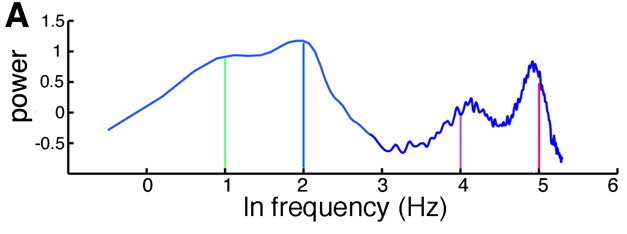
\includegraphics[height=0.4\textheight]{science_2004_f1}
\caption{Power spectrum of hippocampal EEG in the mouse during sleep and waking periods.}
\end{figure}
\end{frame}
\begin{frame}{Example: Coupled Genetic Clocks\cite{Danino:2010aa}}
%\includemovie{.85\textheight}{.85\textheight}{movies/nature08753-s2.mov}
\begin{figure}
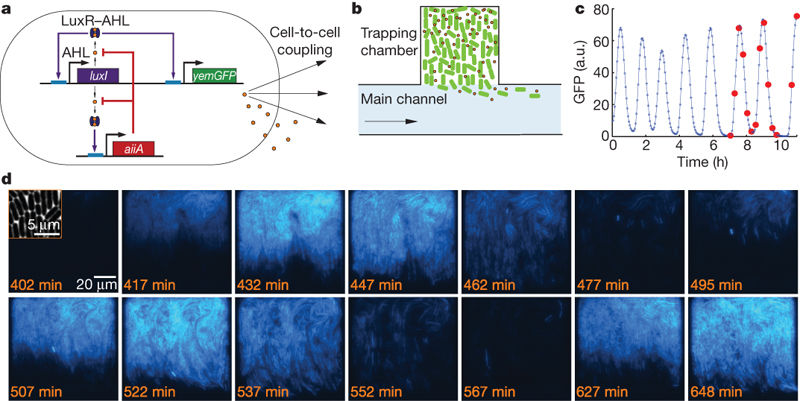
\includegraphics[width=0.95\linewidth]{nature08753-f12}
\end{figure}
\end{frame}
\begin{frame}{A Definition}

\begin{tcolorbox}[notitle, boxrule=0pt, colback=lred]
\centering
	Synchronisation is the process by which weakly\\ interacting oscillatory systems adjust their behaviour\\ to form a collective rhythm.
\end{tcolorbox}
	\begin{columns}
		\scriptsize
	\begin{column}{0.49\textwidth}
		\begin{figure}
			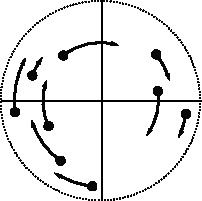
\includegraphics[scale=0.70]{synch1.pdf}
			\caption{Unsynchronised motion: oscillators rotate at different angular velocities.}
		\end{figure}
	\end{column}
	\begin{column}{0.49\textwidth}
		\begin{figure}
			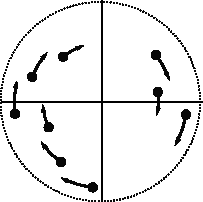
\includegraphics[scale=0.70]{synch2.pdf}
			\caption{Synchronised motion: all oscillators rotate at the same angular velocity.}
		\end{figure}
	\end{column}
\end{columns}
\end{frame}
\begin{frame}{More Examples from biology}
Other examples of biological phenomenon with experimental evidence of synchronisation include\cite{synch}:
\begin{itemize}
	\item Circadian oscillations in cells,
	\item Entrainment of cardiac rhythms,
	\item Ultradian glucose-insulin oscillations in humans,
	\item Glycolytic oscillators in yeast cells,
	\item Predator-prey cycles,
	\item The cell cycle and mitosis in malignant tumors.
	\item Epileptic seizures
\end{itemize}
\end{frame}
\section{Anatomy of a coupled oscillator system}
\begin{frame}{Phenomenological Model of Fireflies}
\begin{minipage}{0.46\textwidth}
\begin{figure}
	\animategraphics[autoplay, loop, width=\linewidth]{3}{anims/fireflies-}{0}{25}
\end{figure}
\end{minipage}\hfill
\begin{minipage}{0.46\textwidth}
With each firefly we associate
\begin{itemize}
	\item an index $j \in 1,\ldots,n$, 
	\item a period between events $T_j$,
	\item a frequency $\omega_j = 2\pi/T_j$,
	\item and a phase $\theta_j \in [0,2\pi)$  such that $\theta_j(t) = \theta_j(t+T_j)$.
\end{itemize}
\end{minipage}

\vspace{15pt}

Some comments:
\begin{itemize}
	\item The natural frequency $\omega_j$ is rarely measurable.
	\item Functions of phase (waveforms) are often measurable.
	\item Noise (both physical and `model' noise) is usually averaged out.
	\item Sometimes amplitudes need also be modelled.
\end{itemize}

\begin{center}
	\vfill
Periodic motion maps really nicely into $\complex$!
\end{center}
\end{frame}

\begin{frame}[t]
\frametitle{Example: Damped harmonic motion in $\complex$.} 
Consider a set (or population) of $n$ damped harmonic oscillators $\{z_j\}$;
\[
\D{z_j}{t} =(-1+\I\omega_j)z_j. \qquad j=1,\ldots,n
\] 
\begin{minipage}{0.49\textwidth}

\vspace{0.5cm}
Each oscillator $z_j$ has:
\begin{itemize}
	\item Phase $\arg{z_j}$,
	\item amplitude $|z_j|$ and 
	\item natural frequency $\omega_j$.
\end{itemize}

Each $\omega_j$ is a real valued I.I.D random variable with density $g(\omega)$.\\

$z_j(t) = z_j(0)\exp[(-1+\I\omega_j)t]$
\end{minipage}
\begin{minipage}{0.49\textwidth}
	\begin{figure}
		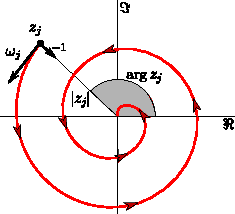
\includegraphics{dosc}
	\end{figure}
	\centering

\end{minipage}
\end{frame}
\begin{frame}
\frametitle{Population mean as a measure of coherence.}
We can measure the state of the population by observing the population mean, or {\em order parameter} \cite{kuramoto75}:
\[
z = \frac{1}{n}\sum_{j=1}^n z_j
\]
\begin{columns}
\begin{column}{0.59\textwidth}
	We call:
	\begin{itemize}
		\item $z$ the {\em mean field}.
		\item $r=|z|$ the mean field amplitude.
		\item $\Theta = \arg{z}$ the mean phase.
		\item $\Omega = \D{\Theta}{t}$ the mean field velocity.
	\end{itemize}
\end{column}
\begin{column}{0.39\textwidth}
	\begin{figure}
		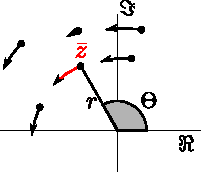
\includegraphics{meanfield.pdf}
	\end{figure}
\end{column}
\end{columns}
\end{frame}
\begin{frame}
\frametitle{Synchronised Vs Unsynchronised Motion}
\begin{figure}
	\animategraphics[autoplay,loop,height=6cm]{6}{anims/lcsynch-}{1}{100}
	\caption{$25$ Oscillators (in red) and the mean field (in blue).}
\end{figure}
\end{frame}
\begin{frame}
\frametitle{A more general model: The Hopf Bifurcation}
The normal form of a Hopf Bifurcation at $\alpha = 0$ is given by
\[
\D{z_j}{t}= (\alpha - \beta|z_j|^2)z_j + \I\omega_j z_j, \qquad \beta >0.
\]
\begin{columns}[t]
\begin{column}{.49\textwidth}
\centering
$\alpha <0$
\begin{figure}
	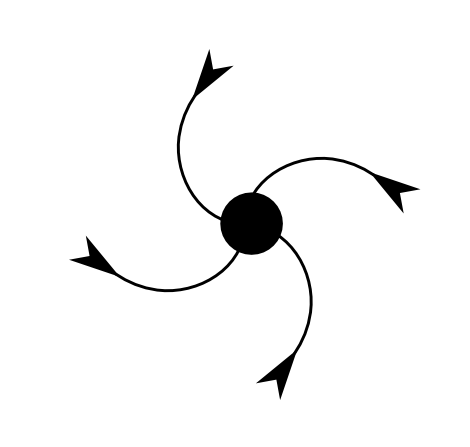
\includegraphics[scale = 0.16]{node.png}
\end{figure}
When $\alpha \le 0$ the fixed point at $z_j =0$ is stable.
\end{column}
\begin{column}{.49\textwidth}
\centering
$\alpha >0$
\begin{figure}
	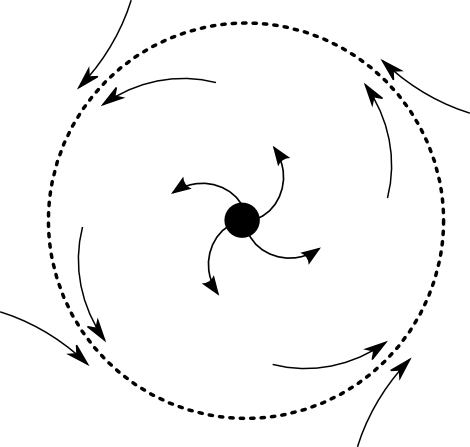
\includegraphics[scale = 0.16]{hopf.png}
\end{figure}
For $\alpha>0$, the $z_j=0$ state is unstable and a stable limit cycle exists with $|z_j| = \sqrt{\alpha/\beta}$				
\end{column}
\end{columns}
\end{frame}
\begin{frame}
\frametitle{Coupled Oscillator Systems on either side of a Hopf}
\begin{columns}[t]
\begin{column}{.49\textwidth}
\centering
Linear Oscillator Model:
\[
\D{z_j}{t} = (\alpha +\I\omega_j)z_j+\Gamma_j(\mathbf{z})
\]
$\alpha <0,\ j = 1\dots n$.
\begin{figure}
	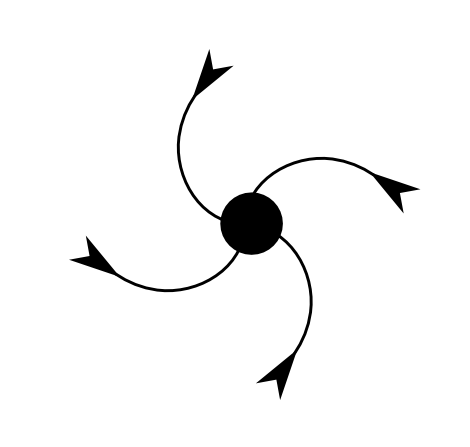
\includegraphics[scale = 0.16]{node.png}
\end{figure}
Decoupled system has a stable node and no stable limit cycles.
\end{column}
\begin{column}{.49\textwidth}
\centering
Limit Cycle Model:
\[
\D{z_j}{t} = (\alpha - \beta|z_j|^2)z_j + \I\omega_jz_j +\Gamma_j(\mathbf{z})
\]
$\alpha,\beta>0, j = 1\dots n$
\begin{figure}
	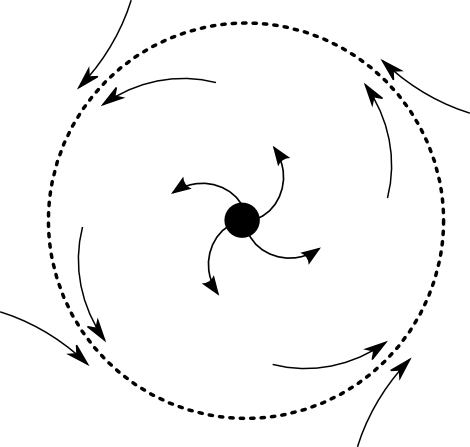
\includegraphics[scale = 0.16]{hopf.png}
\end{figure}
Decoupled system has unstable node and a stable limit cycle.
\end{column}
\end{columns}
\end{frame}
\begin{frame}{The coupling function $\Gamma$}
\[
\quad \D{z_j}{t} = (\alpha - \beta|z_j|^2)z_j + \I\omega_jz_j +\Gamma_j(\mathbf{z}), \qquad j = 1,\ldots, n.
\]
\only<1>{
Network models usually assume linear coupling \[\Gamma_j(\mathbf{z}) = \sum_k w_{jk}z_k.\]
Some common choices include:
\begin{itemize}
	\item All-to-all coupling: $w_{jk} = K/n$
	\item Nearest-neighbour: $w_{jk} = K/n $ iff $(k - j) \mod n = 1$
	\item Small world networks,
	\item Random networks.
\end{itemize}
Nonlinear $\Gamma$ must commute with $\e^{\I \zeta}$. (why?)}
\only<2>{

We restrict ourselves to linear and nonlinear all-to-all coupling of the form
\[
\Gamma(\mathbf{z}) =zF(|z|)=  z(K + K_1|z|^2 + K_2|z|^4 +\ldots) 
\]
where 
\[
z = \frac{1}{n}\sum_{k=1}^nz_k, \qquad K,K_1,\ldots \in \complex
\]
and $F(|z|) \rightarrow 0$ as $|z|\rightarrow \infty$

}
\end{frame}
\begin{frame}{Coupled Limit Cycle Oscillators}
\[
 \quad \D{z_j}{t} = (\alpha - \beta|z_j|^2)z_j + \I\omega_jz_j +\Gamma_j(\mathbf{z}), \qquad j = 1,\ldots, n.
\]
\vfill

To recap:
\begin{itemize}
	\item Oscillators are modelled as points $z_j$ rotating in $\complex$,
	\item $\alpha, \beta$ are fixed parameters,
	\item $\omega_j$ is sampled from a distribution $g(\omega)$,
	\item $\Gamma_j$ is how the oscillator population influences $z_j$,
	\item The mean field $z= \frac{1}{n}\sum_{k=1}^n z_k$ measures coherence.
\end{itemize}
\vfill
\end{frame}
\end{document}